% Opcje klasy 'iithesis' opisane sa w komentarzach w pliku klasy. Za ich pomoca
% ustawia sie przede wszystkim jezyk i rodzaj (lic/inz/mgr) pracy, oraz czy na
% drugiej stronie pracy ma byc skladany wzor oswiadczenia o autorskim wykonaniu.
\documentclass[declaration,inz,english,shortabstract]{iithesis}

\usepackage[utf8]{inputenc}
\usepackage{graphicx}

%%%%% DANE DO STRONY TYTULOWEJ
% Niezaleznie od jezyka pracy wybranego w opcjach klasy, tytul i streszczenie
% pracy nalezy podac zarowno w jezyku polskim, jak i angielskim.
% Pamietaj o madrym (zgodnym z logicznym rozbiorem zdania oraz estetyka) recznym
% zlamaniu wierszy w temacie pracy, zwlaszcza tego w jezyku pracy. Uzyj do tego
% polecenia \fmlinebreak.
\englishtitle   {Formally verified programming with monads in Coq}
\polishtitle    {Formalnie zweryfikowane programowanie z monadami w Coqu}
\polishabstract {Prezentujemy \libname, Coqową bibliotekę do formalnie zweryfikowanego programowania z abstrakcjami w stylu Haskella: funktorami, funktorami aplikatywnymi, monadami, transformatorami monad oraz efektami opartymi o klasy typów. Omawiamy nasze decyzje projektowe, opisujemy implementację i przedstawiamy działanie biblioteki na kilku przykładach.}
\englishabstract{We introduce \libname, a Coq library for formally verified programming with Haskell-style abstractions: functors, applicative functors, monads, monad transformers and typeclass-based effects. We discuss the design choices we made, describe the implementation and illustrate the working of the library on some examples.}
% w pracach wielu autorow nazwiska mozna oddzielic poleceniem \and
\author         {Wojciech Kołowski}
% w przypadku kilku promotorow, lub koniecznosci podania ich afiliacji, linie
% w ponizszym poleceniu mozna zlamac poleceniem \fmlinebreak
\advisor        {dr Maciej Piróg}
\date           {10 września 2019}                     % Data zlozenia pracy
% Dane do oswiadczenia o autorskim wykonaniu
%\transcriptnum {}                     % Numer indeksu
%\advisorgen    {dr. Jana Kowalskiego} % Nazwisko promotora w dopelniaczu
%%%%%

%%%%% WLASNE DODATKOWE PAKIETY
%
%\usepackage{graphicx,listings,amsmath,amssymb,amsthm,amsfonts,tikz}
%\usepackage{minted}
\usepackage{minted}
%
%%%%% WLASNE DEFINICJE I POLECENIA
%
%\theoremstyle{definition} \newtheorem{definition}{Definition}[chapter]
%\theoremstyle{remark} \newtheorem{remark}[definition]{Observation}
%\theoremstyle{plain} \newtheorem{theorem}[definition]{Theorem}
%\theoremstyle{plain} \newtheorem{lemma}[definition]{Lemma}
%\renewcommand \qedsymbol {\ensuremath{\square}}

\newcommand{\libname}{\m{coq-mtl}}
\newcommand{\homepage}{\url{https://github.com/Zeimer/coq-mtl}}

\newcommand{\defn}{:\equiv}
\newcommand{\m}[1]{\texttt{#1}}
\newcommand{\Prop}{\texttt{Prop}}
\newcommand{\Type}{\texttt{Type}}
\newcommand{\nat}{\texttt{nat}}
\newcommand{\Tree}{\texttt{Tree}}

\newcommand{\hintdb}{\m{CoqMTL}}
\newcommand{\hs}{\m{hs}}

%%%%%

\begin{document}

%%%%% POCZATEK ZASADNICZEGO TEKSTU PRACY

\chapter{Introduction} \label{ch1}

This chapter gives some motivations for why formal verification of hardware, software and mathematics is useful and then briefly introduces the Coq proof assistant -- a tool for such verification -- to those who are not familiar with it.

The rest of the thesis is structured as follows:

\begin{itemize}
    \item In \hyperref[ch2]{Chapter 2} we discuss the problem of modeling computational effects in programming languages and compare existing approaches.
    \item In \hyperref[ch3]{Chapter 3} we discuss the design of \libname\ and explain our approach to proof engineering (the formalized mathematics' equivalent of software engineering).
    \item In \hyperref[ch4]{Chapter 4} we describe the implementation, prove a few theorems that assure us of correctness of our abstractions and are useful to ordinary programmers, and show two examples of reasoning about effectful programs.
    \item In \hyperref[ch5]{Chapter 5} we conclude by discussing related and future work.
\end{itemize}

\section{Formal verification of hardware and software}

Since their invention in the 1940s, computers' significance rose at a very fast pace. They were getting applied to an ever expanding range of problems by more and more people, private companies and governments alike. It shouldn't be a considered a surprise then that we became very reliant on them for both small conveniences and large scale projects.

But significance is not the only thing that rose -- another one is complexity. Exponentially growing processing speed required the complexity of chip designs to grow at a similar rate. More complex products and services require more complex software architectures and with new business models, like cloud computing, comes even more complexity in the form of virtualization, containerization and so on.

And with complexity comes, of course, the potential for bugs, which may cause a lot of damage. A malfunction in software running the stock exchange can mean billions of dollars of losses (if not an accidental global recession!); in software running a nuclear power plant -- deadly radiation for thousands of people and energy shortage for millions more.

Due to these dangers a lot of effort has been put into assuring that hardware and software are correct and with great success, but here and there bugs still have crept in. Some of the most spectacular were, recently:

\begin{itemize}
    \item Meltdown, which ``exploits side effects of out-of-order execution on modern processors to read arbitrary kernel-memory locations including  personal  data  and  passwords.'' \cite{Meltdown}
    \item Spectre, which uses speculative execution and branch prediction to ``leak the victim's confidential information via a side  channel to  the  adversary.'' \cite{Spectre}
    \item Heartbleed, which ``allows stealing the information protected, under normal conditions, by the SSL/TLS encryption used to secure the Internet'' \cite{Heartbleed}
\end{itemize}

Academia and industry, however, are not passively waiting for more disasters to happen. DeepSpec \cite{DeepSpec} is a Coq-based project that tries to eliminate both hardware and software bugs and security vulnerabilities by creating a web of formally verified hardware, operating systems, compilers, web servers, cryptography libraries etc. Even though mildly successful already, a long time will pass until it will finally help verify mission-critical real-life systems, like the software running Boeing 737 MAX, which recently caused two such planes to crash \cite{Boeing}.

\section{Formal verification of mathematics}

Hardware and software are not the only things in need of formal verification -- mathematics is also one of them.

The four colour theorem is a problem posed in 1852. It states that any planar map can be coloured with only four colours so that no two regions sharing a boundary are assigned the same colour. It became famous for resisting many proof attempts by many famous mathematicians for more than a century until it was finally proved by Appel and Haken in 1976 \cite{AppelHaken1} \cite{AppelHaken2} \cite{AppelHaken3} \cite{AppelHaken4}. Its importance stems from the proof method -- it was the first major theorem proven using a computer program, whose job was to make sure a very large case analysis was exhaustive.

Thomas Tymoczko, a philosopher of mathematics, criticised this proof by labeling it with a term he invented just for this purpose -- ``non-surveyable'' \cite{NonSurveyable}. He considered a proof to be non-surveyable when its verification cannot be performed by human mathematicians competent in the relevant field. Appel and Haken's proof certainly did fail the surveyability criterion -- the program was written in IBM 370 assembly, a language graph theorists very likely didn't understand.

This was the perfect theorem to let formal proofs and formally verified programs shine by dispelling Tymoczko and other mathematician's doubts. This is what indeed happened in 2005, when Georges Gonthier presented a proof of the theorem formalized in Coq \cite{FourColour1} \cite{FourColour2}.

But big theorems with difficult proofs are not the only call for formalized mathematics. Another one is the mere fallibility of humans, especially their limited memory and reasoning skills and the tendency to follow authority. As unmathematical as it sounds, these are the main reasons cited by Vladimir Voevodsky, a Fields medalist mathematician turned a fan of formal proofs, in one of his talks \cite{UnivalentFoundations}.

The fields he refers to are homotopy theory, higher category theory and motivic cohomology -- all of them containing many layers of abstraction, tons of concepts and definitions, and based on rather shaky foundations (in the sense of foundations of mathematics).

As an example, noticing an error in one of his papers took 7 years and repairing the mistake another 6 years. In another, more extreme case, after publishing a paper in 1989, an alleged counterexample was found in 1998 by another expert in the field, but it was too difficult for them to agree on whether it really was a counterexample and Voevodsky only realized he was wrong in 2013. All of this put him in search of formalized foundations of mathematics, and he chose Coq to purse them. 

\section{The Coq proof assistant}

Coq \cite{Coq} is a proof assistant that was started in the late 1980's in France and is still under active development. It consists of three complementary languages:

\begin{itemize}
    \item Gallina, the term language, implements a formal system whose slight variants go under a plethora of names: Calculus of (Inductive) Constructions, (Intensional) Martin-L\"of Type Theory, Intuitionistic Type Theory, Constructive Type Theory, etc. We can use it to express specifications, programs, theorems and proofs.
    \item Vernacular, the command language, is a language of commands, which allow things like looking up useful theorems in the environment or creating modules.
    \item Ltac, the tactic language, is a language which facilitates writing proofs -- these can in principle be written using the term language, but it's unwieldy even for simple proofs.
\end{itemize}

The basic objects of our interest in Coq (and in any kind of the aforementioned formal systems) are types. Their role is to classify terms -- for example, $\m{21} + \m{21}$ is a term of type \m{nat}, written $\m{21} + \m{21} : \m{nat}$. Types are syntactical entities, which means that the judgment $\m{x} : \m{A}$ can always be checked algorithmically.

Thanks to the the Curry-Howard correspondence \cite{CurryHoward}, types can seen both as specifications of programs and as statements of theorems. All programming and proving may be then conceptualized as manipulating a few kinds of rules:

\begin{itemize}
    \item Formation rules tell us what types are there.
    \item Introduction rules tell us how to construct elements (canonical terms) of a given type.
    \item Elimination rules tell us how to use an element of some type to construct elements of other types.
    \item Computation rules tell us how an elimination rule acts on an introduction rule -- computation happens when we first build something and then take it apart.
    \item Uniqueness rules tell us how an introduction rule acts on an elimination rule -- if we first take something apart and then rebuild it, we should get the same thing we initially had.
\end{itemize}

How does this play out in practice? Let's take a look at an example development, which illustrates the basic workings of Coq. At this point, we strongly encourage the unfamiliar reader to install CoqIDE (a dedicated IDE for Coq, available from \cite{Coq}) and run this snippet (which can be found in the thesis sources in the directory \m{snippets/}) in interactive mode -- this experience will be better than any explanation.

\definecolor{CoqIDE}{RGB}{255,248,220}

\inputminted
[
    frame=lines,
    bgcolor=CoqIDE,
    linenos
]
{Coq}{snippets/snippet1.v}

A Coq file consists of a series of commands, which define types and terms, import and export modules, state or look up theorems etc. In this file we want to implement a function that labels the leaves of a tree with natural numbers starting from $0$.

For this, we will need the type $\m{nat}$, which is provided by the standard library. We can print its definition using the command $\m{Print}$. What we get is an inductive definition of a type with two constructors, $\m{O}$ and $\m{S}$. $\m{O}$ is supposed to represent $0$ and $\m{S}$ is supposed to represent the successor operation, so that $\m{S}\ \m{O}$ represents $1$, $\m{S}\ (\m{S}\ \m{O})$ represents $2$ and so on.

We will also need a type $\m{Tree}$ that represents trees. The definition will be inductive, just as for natural numbers, but this time is has a parameter $A : \m{Type}$ that tells us the type of elements that can be stored in the tree. This can be seen as defining infinitely many types at once -- one for each choice of $A$. There are two constructors: $\m{Leaf}$, which represents a tree with one element, and $\m{Node}$, which represents a tree with two subtrees. Thus our trees are always nonempty and they contain elements only in their leaves.

The next two commands, \m{Arguments}, control the use of implicit arguments. Normally, we would have to write $\m{Leaf}\ \nat\ 42$ for the tree containing only the value $42$, but this is redundant, since given a term like $\m{42}$, we can infer its type to be $\nat$. We can thus write this as $\m{Leaf}\ \_\ \m{42}$, but this is still redundant. Thanks to the first of these two commands, we can write simply $\m{Leaf}\ \m{42}$. The second command has a similar effect on the other constructor, \m{Node}.

The function \m{label} is the clou of the whole development. It's type says that given a type \m{A} (which we won't need to give explicitly, since it's an implicit argument, thanks to the curly braces), a tree \m{t} that holds elements of type \m{A} and a natural number \m{n} which acts as the counter, it returns a pair consisting of a natural number (the new counter) and a tree containing elements of type $\m{A} * \nat$.

The definition is recursive (marked by the keyword \m{Fixpoint}). When we hit a \m{Leaf}, we return the current counter and label the leaf with the counter's value. When we encounter a \m{Node}, we label the left subtree using the current counter, then label the right subtree with the new counter incremented by one, and then return the new counter and the two labeled subtrees joined by the constructor \m{Node}. We can use this auxiliary function to define \m{lbl}, the function we wanted from the very beginning.

The command \m{Compute} normalizes a given term, which in type-theoretical parlance means just running a computation (which in Coq is guaranteed to finish). In our case, we run \m{lbl} on an example tree to see that the result is as we expected -- the leaves are now labeled with natural numbers, starting at zero, from left to right.

But how do we prove what we have done really is what we intended? The basic approach is to invent some properties we would like our program to satisfy. If it does satisfy all of these desired properties and they encapsulate everything we require from the program's behaviour, we may consider the program correct for our purposes.

In our case, one simple property is that after labeling a tree \m{t} the counter increases by the size of the tree minus one. To state this property formally, we first need to define a function that computes the size of a tree. We do this by recursion: a \m{Leaf} has size $1$ and the size of a \m{Node} is the sum of sizes of its subtrees.

The command \m{Require Import} imports a module. To prove our theorem, we will need some simple theorems about addition and multiplication of natural numbers, which we can find in a module called \m{Arith}.

Now we are ready to state our theorem. It reads: for any type \m{A}, any \m{t} which is a tree of elements of type \m{A}, any two natural numbers \m{n} and \m{n'} and any \m{t'} which is a tree of elements of type \m{A * nat}, if calling label on \m{t} and \m{n} results in the pair \m{(n', t')}, then the successor of \m{n'} is equal to \m{n + size\ t}.

There are some points to be noticed. First, we quantify over types, which means that our logic is not first-order, but higher-order. Second, we need to quantify over \m{t'}, even though the tree resulting from the call to label is of no interest to us. Third, we avoid using subtraction or the predecessor function and instead express our theorem using successor. This is a technicality -- our theorem will be a bit easier to prove this way.

We now enter the proof mode, in which we can use tactics to prove our theorem. The command \m{Proof} is useless, because it does nothing, but it looks nice at the beginning of a proof.

We proceed by induction on \m{t}. The clause \m{as [| l IHl r IHr]} allows us to name variables and induction hypotheses. This may seem weird to a classically-minded mathematician, but is actually an important aspect of proof engineering -- to make our proofs readable and resilient to change, it's a good practice to name variables and hypotheses manually (as opposed to using automatically generated names).

To boost the unfamiliar reader's curiosity and encourage him to see the proof in CoqIDE, we will not go over it in detail. It suffices to say that the in first case the result holds almost by computation, but we need to use the commutativity of addition and in the second case we basically just use our two inductive hypotheses and the associativity of addition.

This concludes our introduction to the Coq proof assistant. From now on we will assume that the reader is familiar with it. If that's not the case, there are a great many of books which make a good introduction:

\begin{itemize}
    \item Software Foundations \cite{SoftwareFoundations} is a four volume book by many authors. The first volume treats the basics of Coq and the third one is about formally proving correctness of algorithms in Coq. The second and fourth volumes are less relevant, as they are about formalizing programming languages and randomized testing, respectively.
    \item Coq'Art \cite{CoqArt} is a comprehensive but a little dated (2004) book that covers way more material than Software Foundations, including coinduction, proof by reflection, case studies and so on.
    \item Certified Programming with Dependent Types \cite{CPDT} is an advanced book that focuses on using dependent types and proof engineering, but also covers topics like axioms, reasoning about equality proofs and general recursion.
\end{itemize}

\chapter{Effects} \label{ch2}

Although \libname\ started as a rather general-purpose library, it mainly tackles the problem of how to best express (and program with) effects. The research on effects is still young and active, so in this chapter we will take a look at the basic concepts to gain some familiarity with it. However, to keep the exposition accessible to ordinary programmers, our treatment will be rather loose and hands-on.

\section{Basic concepts}

A \textbf{side effect} is some kind of communication with the outside world, like:

\begin{itemize}
    \item Reading external configuration.
    \item Logging to a file.
    \item Pseudorandomness, because it requires a seed.
    \item Any kind of IO, like connecting to the Internet or querying a database.
    \item Memory management, like allocation and freeing.
    \item Concurrency and threads, because they need some kind of synchronization, either through shared memory or message passing.
\end{itemize}

An \textbf{effect} (sometimes also called a \textbf{computational effect}) is either a side effect or use of some control mechanism, like:

\begin{itemize}
    \item Generators and coroutines.
    \item Nondeterminism: the computation may return multiple results.
    \item Partiality: the computation may return \m{null} or some similar value representing the lack of result.
    \item Exceptions: the computation may fail by throwing an exception, which may or may not then be handled by some other computation.
    \item Goto: the computation may pass control to some other computation.
    \item Continuations: the most general control mechanism, which can express all of the above ones.
    \item Sometimes nontermination and even termination are also considered effects, but that's a tougher topic, beyond the scope of this thesis.
\end{itemize}

It should be quite obvious that effects are useful. They are in fact the main reason for running most computer programs and without them running even the simplest number-crunching program would be pointless, since without IO operations it couldn't tell us the result. We thus want to be able to express effects. But we also want to be able to reason about our effectful programs, which in most programming languages is notoriously difficult, and moreover we want to verify our reasoning.

\section{A comparison}

To better understand the matter, we can classify all expressions in a programming language as being either values or computations. A \textbf{value} necessarily has no effects whereas a \textbf{computation} may have effects. Philosophically, we say that a value is but a computation does. We can then say that a language is \textbf{pure} when it explicitly separates values from computations and \textbf{impure} when it does not.

When interpreted as a yes-no property, most languages are impure, so it is better to see the concept of purity as a continuum, where some languages may be more pure than others. Let's examine a few real-world languages and see, where they can be placed on this continuum.

C is a very impure language. There is global state in the form of global variables. Even though ``considered harmful'', we can use the \m{goto} statement anywhere, just as IO operations. It's fair to say that C certainly does not even try to separate values from computations.

In Java, there's no global state, but objects still have internal state that methods can change. There's no \m{goto} and some exceptions are checked, which makes them apparent in type signatures. But there also are unchecked exceptions that don't appear in type signatures and IO operations may be used anywhere. Thus, even though there are some ad hoc attempts at separating values from computations (checked exceptions), Java still can't do this in a principled way. It is still an impure language, though less than C.

Haskell, on the other hand, is a reasonably pure language. There is no global state. There's an impure error mechanism, but it is barely used and usually replaced with explicit error handling. IO can be used anywhere by using functions like \m{unsafePerformIO}, but this can't be done accidentally and is generally avoided. Therefore, nearly all error handling and IO and all other effects are expressed using monads, which are clearly visible in type signatures and make values and computations very easy to tell apart. This is the reason that Haskell is generally perceived as a pure language.

At last, Koka \cite{Koka} is one of the purest languages in existence. It clearly separates values from computations -- each expression, besides its type, is also assigned the list of all effects that it may produce and even nontermination is tracked this way. The tracking is performed by the effect system and is an integral part of Koka's design. This may be contrasted with Haskell, where monads are a library-level concept and the language was not designed with the value-computation distinction in mind.

To better see these differences, let's look at a piece of code that loops before trying to print something to the screen in each of these four languages.

\begin{listing}[H]
    \begin{minted}{C}
        void f()
        {
            f();
            printf("Effectful\n");
        }
    \end{minted}
    \caption{C}
\end{listing}

\begin{listing}[H]
    \begin{minted}{Java}
        public void f()
        {
            f();
            System.out.println("Effectful");
        }
    \end{minted}
    \caption{Java}
\end{listing}

\begin{listing}[H]
    \begin{minted}{Haskell}
        f :: IO ()
        f = do
            f
            putStrLn "Effectful"
    \end{minted}
    \caption{Haskell}
\end{listing}

\begin{listing}[H]
    \begin{minted}{Koka}
        function f() : <div, io> ()
        {
            f()
            println("Effectful")
        }
    \end{minted}
    \caption{Koka}
\end{listing}

We see that in C and Java the return type is just \m{void}, which in these languages represents a type with only one value. There is no type-level indication whatsoever that these programs perform any kind of side effects.

In Haskell, the type is \m{IO ()}, where \m{()} is analogous to \m{void} and \m{IO} indicates that an IO operation. The \m{IO} part can't be omitted in the type of \m{f}, because the type of \m{putStrLn} is \m{String -> IO ()}.

In Koka, the return type is also \m{()}, which is analogous to Haskell's \m{()} and C and Java's \m{void}, but the signature also contains the row of effects \m{<div, io>}, which indicates that \m{f} can loop or perform IO operations.

We can see that, even though at their foundations those four languages are quite different from each other, C and Java cluster together at the impure end of the spectrum, whereas Haskell and Koka, despite their effect systems being different, cluster together at the pure end.

\section{Approaches to effect systems}

An \textbf{effect system} is a means of carrying out the separation of values and computations. In the previous section we have already seen two approaches to effect systems, but before taking a closer look at them, we should first ask whether it is beneficial to have an effect system. This question is best answered by Tony Hoare, who invented quicksort, Hoare logic, Communicating Sequential Processes and also the worst nightmare of many programmers, the null reference \cite{BillionDollarMistake}:

\begin{quote}
    I call it my billion-dollar mistake. It was the invention of the null reference in 1965. At that time, I was designing the first comprehensive type system for references in an object oriented language (ALGOL W). My goal was to ensure that all use of references should be absolutely safe, with checking performed automatically by the compiler. But I couldn't resist the temptation to put in a null reference, simply because it was so easy to implement. This has led to innumerable errors, vulnerabilities, and system crashes, which have probably caused a billion dollars of pain and damage in the last forty years
\end{quote}

This ``billion dollar mistake'' is only the tip of the iceberg of allowing effects without properly tracking them (references allowing nulls can be seen as a kind of ``missing value'' effect). It isn't too hard to imagine that other effects  can cause even more problems. For example, if a function throws an exception without this being indicated in the type signature, the client code may forget to handle it.

The problem of null references is easily fixed with some kind of effect system. For example, we could require all references to be non-null and introduce a special option type to represent missing values. Then references which can be ``null'' can be statically differentiated from those that cannot by the type system.

After seeing some anecdotal evidence supporting the superiority of having an effect system, we are ready to see the contending approaches.

\subsection{Monads, transformers and typeclasses}

The oldest approach, which is quite ad hoc, amounts to implementing monads and various related structures at the library level and using them to track effects using the type system. This approach can be called the \m{mtl} approach, after a Haskell library that implements it.

Monads were initially invented by category theorists in the 1960s for the purpose of universal algebra and named after a concept coming from the philosophy of Leibniz. A running joke in the functional programming community (based on an actual quote from \cite{CWM}) is that

\begin{quote}
    A monad in $C$ is just a monoid in the category of endofunctors of $C$, with product $\times$ replaced by composition of endofunctors and unit set by the identity endofunctor. What's the problem?
\end{quote}

Despite their current reputation of being hard to understand (at least for ordinary programmers \cite{MonadTutorialFallacy}), Moggi realized in his famous 1991 paper \cite{Moggi} that they are in fact quite a simple abstraction that can be used to represent effects. Namely, a \textbf{monad} $M : \Type \to \Type$ is a function from types to types, and $M\ A$ may be interpreted as the type of computations that return a value of type $A$, but which may have an effect represented by $M$.

Each monad has an operation $\m{pure} : A \to M\ A$ which turns a value into an effectless computation and an operation $\m{bind} : M\ A \to (A \to M\ B) \to M\ B$, which runs the first computation and feeds its result to a function that uses it to produce another computation. These operations are related by laws that are monoid laws in disguise.

Monads, however, are not the silver bullet of effectful programming and come bundled not only with operations, but also with problems. The most obvious problem is that a monad represents a single effect, but we of course want to have multiple effects at once. Implementing a new monad for each desirable combination of effects is not a sane option and this causes us to search for a way of composing monads.

Such a way of composing monads are monad transformers \cite{mtl}. A \textbf{monad transformer} \m{T} is an object of type $\m{T} : (\Type \to \Type) \to (\Type \to \Type)$ that represents an effect and $\m{T}\ \m{M}\ \m{A}$ (\m{T} applied to a monad \m{M} and a type \m{A}), represents a type of computations that return a value of type \m{A} but may also perform effects represented by \m{T} and \m{M}. It comes bundled with an operation $\m{lift} : \m{M}\ \m{A} \to \m{T}\ \m{M}\ \m{A}$ that turns a computation that can have only one kind of effect into one that can have two.

Transformers \m{T} and \m{S} and a monad \m{M} can then be composed to give a monad $\m{T}\ (\m{S}\ \m{M})$. Because each monad has its corresponding transformer, we can get rid of all the monads (except for one, the identity monad) and use just the transformers.

Monad transformers, even though they solve the problem of composing monads, come with their own problems too. The simplest and most annoying
is the fact that for complicated transformer stacks we need to use the \m{lift} operation a lot. For example, we would need two \m{lift}s to get from $\m{M}\ \m{A}$ to $\m{T}\ (\m{S}\ \m{M})\ \m{A}$. This is a rather annoying problem, because real-world code often requires way more than just two effects.

This deficiency can be remedied by introducing a more abstract design based on describing effects with \textbf{typeclasses} \cite{mtl}, which are basically the same thing as interfaces. Here each effect \m{E} is split into a specification and an implementation. The specification is a typeclass that expresses \m{E} by listing the operations that it supports. For example, the state effect supports \m{get} to retrieve the current state and \m{put} to modify the state. That a particular monad \m{M} supports the effect \m{E} is then expressed by implementing an instance of this typeclass for the monad \m{M}.

This solves the problem with too many \m{lift}s, but still has its own problems. One is that the number of implementations required is quadratic, because usually each transformer needs to implement each typeclass. However, in practice this is not as big a problem as having to implement a separate monad for each combination of effects.

Another problem, far bigger and more conceptual, is the ordering of effects: if a monad is both stateful and nondeterministic, how do these two effects interact? Is there a global shared state or does each branch of the computation have its own local state?

\subsection{Algebraic effects and handlers}

These problems with effect ordering suggest the idea that maybe there shouldn't be a static ordering. Maybe the meaning of combinations of effects, like state + nondeterminism, shouldn't be fixed ahead of time? Ultimately, maybe even the meaning of the effects themselves shouldn't be fixed?

This leads to a refinement of the notion of effect specification, which ceases to be an interface describing the operations associated with the effect and becomes an algebraic data type that represents these operations. Thus these new effects can be called \textbf{algebraic effects}, but there is more to this name than just the algebraicness of the data types.

This change prompts a refinement of the notion of implementation of an effect. Instead of simply being a monad transformer, an implementation of an effect is now an \textbf{effect handler} -- an operation that takes an effectful computation as input and transforms it into another computation. We can use handlers to realize an effect in some concrete way, translate the effect into some other effect or even throw the effect away.

For example, when we have a ``log'' effect and a ``debug'' effect, our production code can realize logging using some logging service and discard the debugging effect while our test code can do exactly the opposite! Handlers can be useful for testing in an even more general way: the test code can interpret effects by mocking them, which is a very popular unit testing technique in the object-oriented programming world.

Algebraic effects and handlers come in two flavours. One of them is to implement these abstractions at the library level using some new concepts like free monads or open unions, but also relying on the old menagerie of monads and monad transformers. This approach can be called \m{extensible-effects} after a Haskell library that proposed it. \cite{ExtensibleEffects} \cite{Freer}

The second flavour, the most recent and promising one, represented by languages such as Koka \cite{Koka}, Eff \cite{Eff}, Frank \cite{Frank}, Multicore OCaml \cite{MulticoreOCaml} and Helium \cite{Helium}, instead aims to implement support for programming with algebraic effects and handlers at the language level, which has many practical advantages.

Native treatment of effects allows special treatment during compilation, which results in better performance. Integrating effect checking and effect inference with type checking and type inference results in better error messages and more manageable function signatures. Built-in support for effectful computations means lighter syntax and less boilerplate -- for example, Haskell style \m{do}-notation is no longer needed, and built-in support for effect definitions means it is way easier to implement a custom effect than with \m{extensible-effects}, which requires one to dive a little into the library internals.

But probably the greatest advantage of this approach is its conceptual simplicity. Both \m{mtl} and \m{extensible-effects} suffer from a plethora of closely related concepts: monads and monad transformers, free and free-er monads, their operations and laws, the idea that they (indirectly) represent effects, and on top of it typeclasses, which are quite orthogonal to the subject at hand. This can be contrasted with the conceptual simplicity of native algebraic effects, with just the two core concepts of effects and handlers.

In my opinion, this conceptual simplicity is crucial for industry adoption -- if the average Java programmer can't understand the basic ideas behind effects, there will be no wide adoption and thus no benefits from reduced number of bugs.

\chapter{Design} \label{ch3}

In this chapter we describe the design of \libname. We motivate the library's design by discussing possible ways of implementing effects in Coq, design choices related to abstraction and modularity mechanisms, various ways of using classes for formalizing concepts, and the matter of axioms.

\section{Effects in Coq?}

Now that we know the basics of effects, we can decide on how to best implement them in Coq.

First off, we need to recall that Coq implements Calculus of Inductive Constructions. This variant of type theory was not designed with the value-computation distinction in mind. Because of this, any native support of effects is ruled out -- this would amount to implementing a whole new language, not to mention that such a language would have to be invented first - for example, at present no variant of type theory has both algebraic effects and dependent types.

Then we should ask ourselves, why do we want to have a way of expressing effects in Coq? After all, Coq is a proof assistant concerned mainly with theorem proving and formal verification that doesn't even support any kind of IO -- you can't use it to write the simplest Hello World program, you can't connect to a database, you can't use it to write a web server (but see \cite{CoqIO}).

We can answer this by recalling that effects are not only about communication with the outside world -- they can also model control mechanisms like failure, exceptions or nondeterminism, and we surely want to make programming with these easier. The function \m{label} we saw at the end of \hyperref[ch1]{Chapter 1} could look way better expressed using the state effect.

Another reason is that, even though in Coq we can't interact with the outside world, we may want to model programs or programming languages that can. At last, IO and other such effects may be added to Coq in the future and we want to be prepared for that (related languages, like Agda \cite{Agda} and Idris \cite{Idris} both have IO).

We are thus forced to implement our effects at the library level and because the \m{extensible-effects} approach depends crucially on many \m{mtl} abstractions as described earlier, we choose to implement the latter and leave the former for future work.

\section{Typeclasses, canonical structures and modules}

The good news is that Coq has various mechanisms for achieving abstraction and modularity, such as typeclasses, canonical structures and modules. The bad news is that these mechanisms are related, overlapping, and their use inside the standard library and in third party libraries is not very consistent. We will therefore try to explain the similarities and differences motivating our choice of using typeclasses to implement the library.

Typeclasses \cite{Classes1} \cite{Classes2} were originally invented for the purpose of overloading arithmetical operators in Haskell, but since then they were found to have many more applications and spread to other languages, like Rust.

In Coq, typeclasses are basically parametrized dependent records (collections of fields where types of later fields can depend on values of earlier fields and all of the fields can depend on the parameters) together with the mechanism of instance search (implemented using ordinary proof search) and a priority mechanism for deciding between overlapping instances. Listing \ref{SgrClass} shows an example use of typeclasses to formalize a semigroup, a very simple algebraic structure that consists of a type together with an associative binary operation.

\begin{listing}[H]

\begin{minted}
[
    frame=lines,
    bgcolor=CoqIDE,
    linenos
]{Coq}
    
Class Semigroup (A : Type) : Type :=
{
    op : A -> A -> A;
    assoc : forall x y z : A, op (op x y) z = op x (op y z);
}.

\end{minted}

\caption{Semigroups represented with typeclasses}
\label{SgrClass}

\end{listing}

Canonical structures are a mechanism unique to Coq. They were introduced in a 1998 PhD thesis in French \cite{CanonicalStructures0} and remain quite obscure since then, but there were some attempts at explaining them better \cite{CanonicalStructures1} \cite{CanonicalStructures2} \cite{CanonicalStructures3}. They are built on the foundation of parametrized dependent records, just like typeclasses, but they differ from the latter in the instance search mechanism -- canonical structures are found using unification and not ad hoc proof search.

They also lack native handling of overlapping instances and backtracking, but this can be remedied with some hacks (see the conclusion section of \cite{CanonicalStructures2} for a detailed comparison of typeclasses and canonical structures). They are usually coupled with the module mechanism -- this approach is well present in the Mathematical Components library \cite{MCB}, a spin-off of the formalization of the Four Colour Theorem \cite{FourColour1} \cite{FourColour2}. Listing \ref{SgrCS} shows a formalization of semigroups using canonical structures.

\begin{listing}[H]

\begin{minted}
[
    frame=lines,
    bgcolor=CoqIDE,
    linenos
]{Coq}

Module Semigroup.

    Record class (A : Type) := Class
    {
        op' : A -> A -> A;
        assoc : forall x y z : A, op' (op' x y) z = op' x (op' y z);
    }.

    Structure type := Pack
    {
        obj : Type;
        class_of : class obj;
    }.

    Definition op (e : type) : obj e -> obj e -> obj e :=
    let 'Pack _ (Class _ op' _) := e in op'.

    Arguments op {e} x y : simpl never.
    Arguments Class {A} op'.

End Semigroup.

\end{minted}

\caption{Semigroups represented with canonical structures (and modules)}
\label{SgrCS}

\end{listing}

The last of Coq's abstraction mechanisms is the module system \cite{Modules1} \cite{Modules2}, inspired by the module system of ML. Modules, just like typeclasses and canonical structures, are very similar to parametrized dependent records (though not implemented using them), but they are less restrictive, because the body of a module can also contain vernacular commands, like inductive type definitions.

It is precisely these inductive type definitions that forbid Coq modules from being first-class (it may come as a surprise, but defining a new type can be considered an effect, because new named constants are added into the environment). Modules are also often used as namespaces, because all names declared in a module must be accessed by prefixing them with the module name, unless the module is imported into scope. Listing \ref{SgrModule} shows a formalization of semigroups using modules (or, to be more precise, module types).

\begin{listing}[H]

\begin{minted}
[
    frame=lines,
    bgcolor=CoqIDE,
    linenos
]{Coq}

Module Type Semigroup.

    Parameter A : Type.
    Parameter op : A -> A -> A.
    Axiom assoc :
        forall x y z : A, op (op x y) z = op x (op y z).

End Semigroup.

\end{minted}

\caption{Semigroups represented with modules}
\label{SgrModule}

\end{listing}

Listings \ref{SgrClass}, \ref{SgrCS} and \ref{SgrModule} all look very much alike, except that the solution using canonical structures is longer, because one usually formalizes both the bundled and unbundled version of the concept (see next section for explanation).

Our abstraction and modularity mechanism of choice were typeclasses. The most important reason was that we wanted the library to be intelligible to people with Haskell background. An additional motivation was that the only other work on monads in Coq \cite{MERC} uses canonical structures, so we wanted to try something different.

\section{Bundles, outlaws, setoids and other exotic animals}

Choosing typeclasses as our abstraction mechanism doesn't exhaust the design space yet. In comparison to Haskell's, Coq's typeclasses are way more powerful, as they are both first-class and higher-order. For example, in Coq we can have functions which take functions between typeclasses as inputs and return functions between typeclasses as outputs, whereas in Haskell such constructions are not allowed. This particular example is a bit artificial, but when implementing a class hierarchy in Coq, there are at least three additional design choices that we can make which are not available in Haskell.

\begin{listing}[H]

\begin{minted}
[
    frame=lines,
    bgcolor=CoqIDE,
    linenos
]{Coq}

Class Semigroup : Type :=
{
    A : Type;
    op : A -> A -> A;
    assoc : forall x y z : A, op (op x y) z = op x (op y z);
}.

\end{minted}

\caption{The bundled approach}
\label{Bundled}

\end{listing}

\begin{listing}[H]

\begin{minted}
[
    frame=lines,
    bgcolor=CoqIDE,
    linenos
]{Coq}

Class Semigroup (A : Type) : Type :=
{
    op : A -> A -> A;
    assoc : forall x y z : A, op (op x y) z = op x (op y z);
}.

\end{minted}

\caption{The unbundled approach}
\label{Unbundled}

\end{listing}

The first one I will call bundling. A bundled class is one that has no parameters -- all the aspects of the concept being formalized are represented using fields. An example is shown in listing \ref{Bundled}. An unbundled class is one where some of the fields were moved to become parameters instead, as shown in listing \ref{Unbundled}. A class can be unbundled to various degrees -- in our example, we have only unbundled the type \m{A}, but we could have also unbundled the operation \m{op} (or even the law \m{assoc}, but that would be silly).

The bundled approach is better when we are interested in treating our concepts as objects on which we will operate. The unbundled approach is better when we want to use typeclasses as interfaces, which link the class parameters to its fields. Another advantage of the unbundled approach is that we can put an unbundled class together with its parameters in a new class (in a way very similar to that from listing \ref{SgrCS}) to recover the bundled version of this class. The other way around (recovering an unbundled class from its bundled version) is harder. We will therefore follow the unbundled approach.

\begin{listing}[H]

\begin{minted}
[
    frame=lines,
    bgcolor=CoqIDE,
    linenos
]{Coq}

Class Semigroup : Type :=
{
    A : Type;
    op : A -> A -> Type;
}.

Coercion A : Semigroup >-> Sortclass.

Class SemigroupLaws (S : Semigroup) : Prop :=
{
    assoc : forall x y z : S, op (op x y) z = op x (op y z);
}.

Class LawfulSemigroup : Type :=
{
    sgr : Semigroup;
    laws : SemigroupLaws sgr;
}.

\end{minted}

\caption{The (bundled) lawless approach}
\label{Lawless}

\end{listing}

Another approach to class design, whose example is shown in listing \ref{Lawless}, I will call the lawful/lawless approach. The idea is a bit similar to bundling/unbundling: a lawful class is one that contains all the relevant laws, whereas in the lawless approach we split a class into two: the ``main'' class with all the data and operations and the ``laws'' class that contains all the (equational or other) laws that these data and operations should satisfy.

There are a few reasons why one might want to split laws from the main class. First, we may be interested in how fast the resulting code will execute in Coq (and not only after extraction), and carrying around proofs of all the laws and computing with them may slow down the execution speed. Second, we might want users of our classes to be able to program without having to prove anything at all. Third, we might be interested in proving some nontrivial properties, like equivalence of various classes (we will do this in \hyperref[ch4]{Chapter 4}), in which case having to prove equality of proofs of the laws might be notoriously annoying or even require introducing an additional axiom -- the Proof Irrelevance Axiom.

For \libname\ we adopt the lawful approach because we are interested not in programming per se, but in formally verified programming. In practice, it turns out that the lawful approach doesn't have a big impact on execution speed. Since we are interested in proving typeclass equivalences for practical purposes (to allow the programmer to implement what's easiest for him but get everything), we don't need to do deal with proof equality in our proofs.

\begin{listing}[H]

\begin{minted}
[
    frame=lines,
    bgcolor=CoqIDE,
    linenos
]{Coq}

Class Setoid : Type :=
{
    carrier : Type;
    eqv : carrier -> carrier -> Prop;
    refl : forall x : carrier, eqv x x;
    sym : forall x y : carrier, eqv x y -> eqv y x;
    trans : forall x y z : carrier, eqv x y -> eqv y z -> eqv x z;
}.

Coercion carrier : Setoid >-> Sortclass.

Class Semigroup : Type :=
{
    A : Setoid;
    op : A -> A -> A;
    assoc : forall x y z : A, eqv (op (op x y) z) (op x (op y z));
    op_eqv : forall x x' y y' : A,
                eqv x x' -> eqv y y' -> eqv (op x y) (op x' y');
}.

\end{minted}

\caption{The (bundled) setoid approach}
\label{Setoid}

\end{listing}

The last thing we could do is using setoids instead of types to formalize the concepts of interest. A setoid is a type together with an equivalence relation and this approach boils down to replacing all types with setoids and adding the necessary compatibility laws for operations, as shown in listing \ref{Setoid}.

The main use of setoids is in dealing with equality -- because we cannot form quotient types in Coq, any kind of mathematics that requires quotients (algebra), gluing (topology), or just simply changing the notion of equality for a particular structure, needs to be carried out using setoids. We would need to use them if we wanted to focus on the category-theoretical aspects of monads and monad transformers, but since we are interested mainly in the practical aspects, we will not need any setoids.

To sum it up, bundled classes are best used for formalizing mathematics, with setoids when in need of quotients/gluing, whereas unbundled classes are best used for representing interfaces, possibly without the laws if we care only about programming and not proving.

\subsection{The final class hierarchy}

The choices we made mostly exhaust the design space. All other basic basic design choices (the class hierarchy up to monad transformers, naming of modules and functions, etc.) were made to match Haskell. Together with the monadic effect classes taken from \cite{JustDoIt}, this results in the hierarchy of classes and their instances shown in figure \ref{fig:hierarchy}.

\begin{figure}
    \centerline{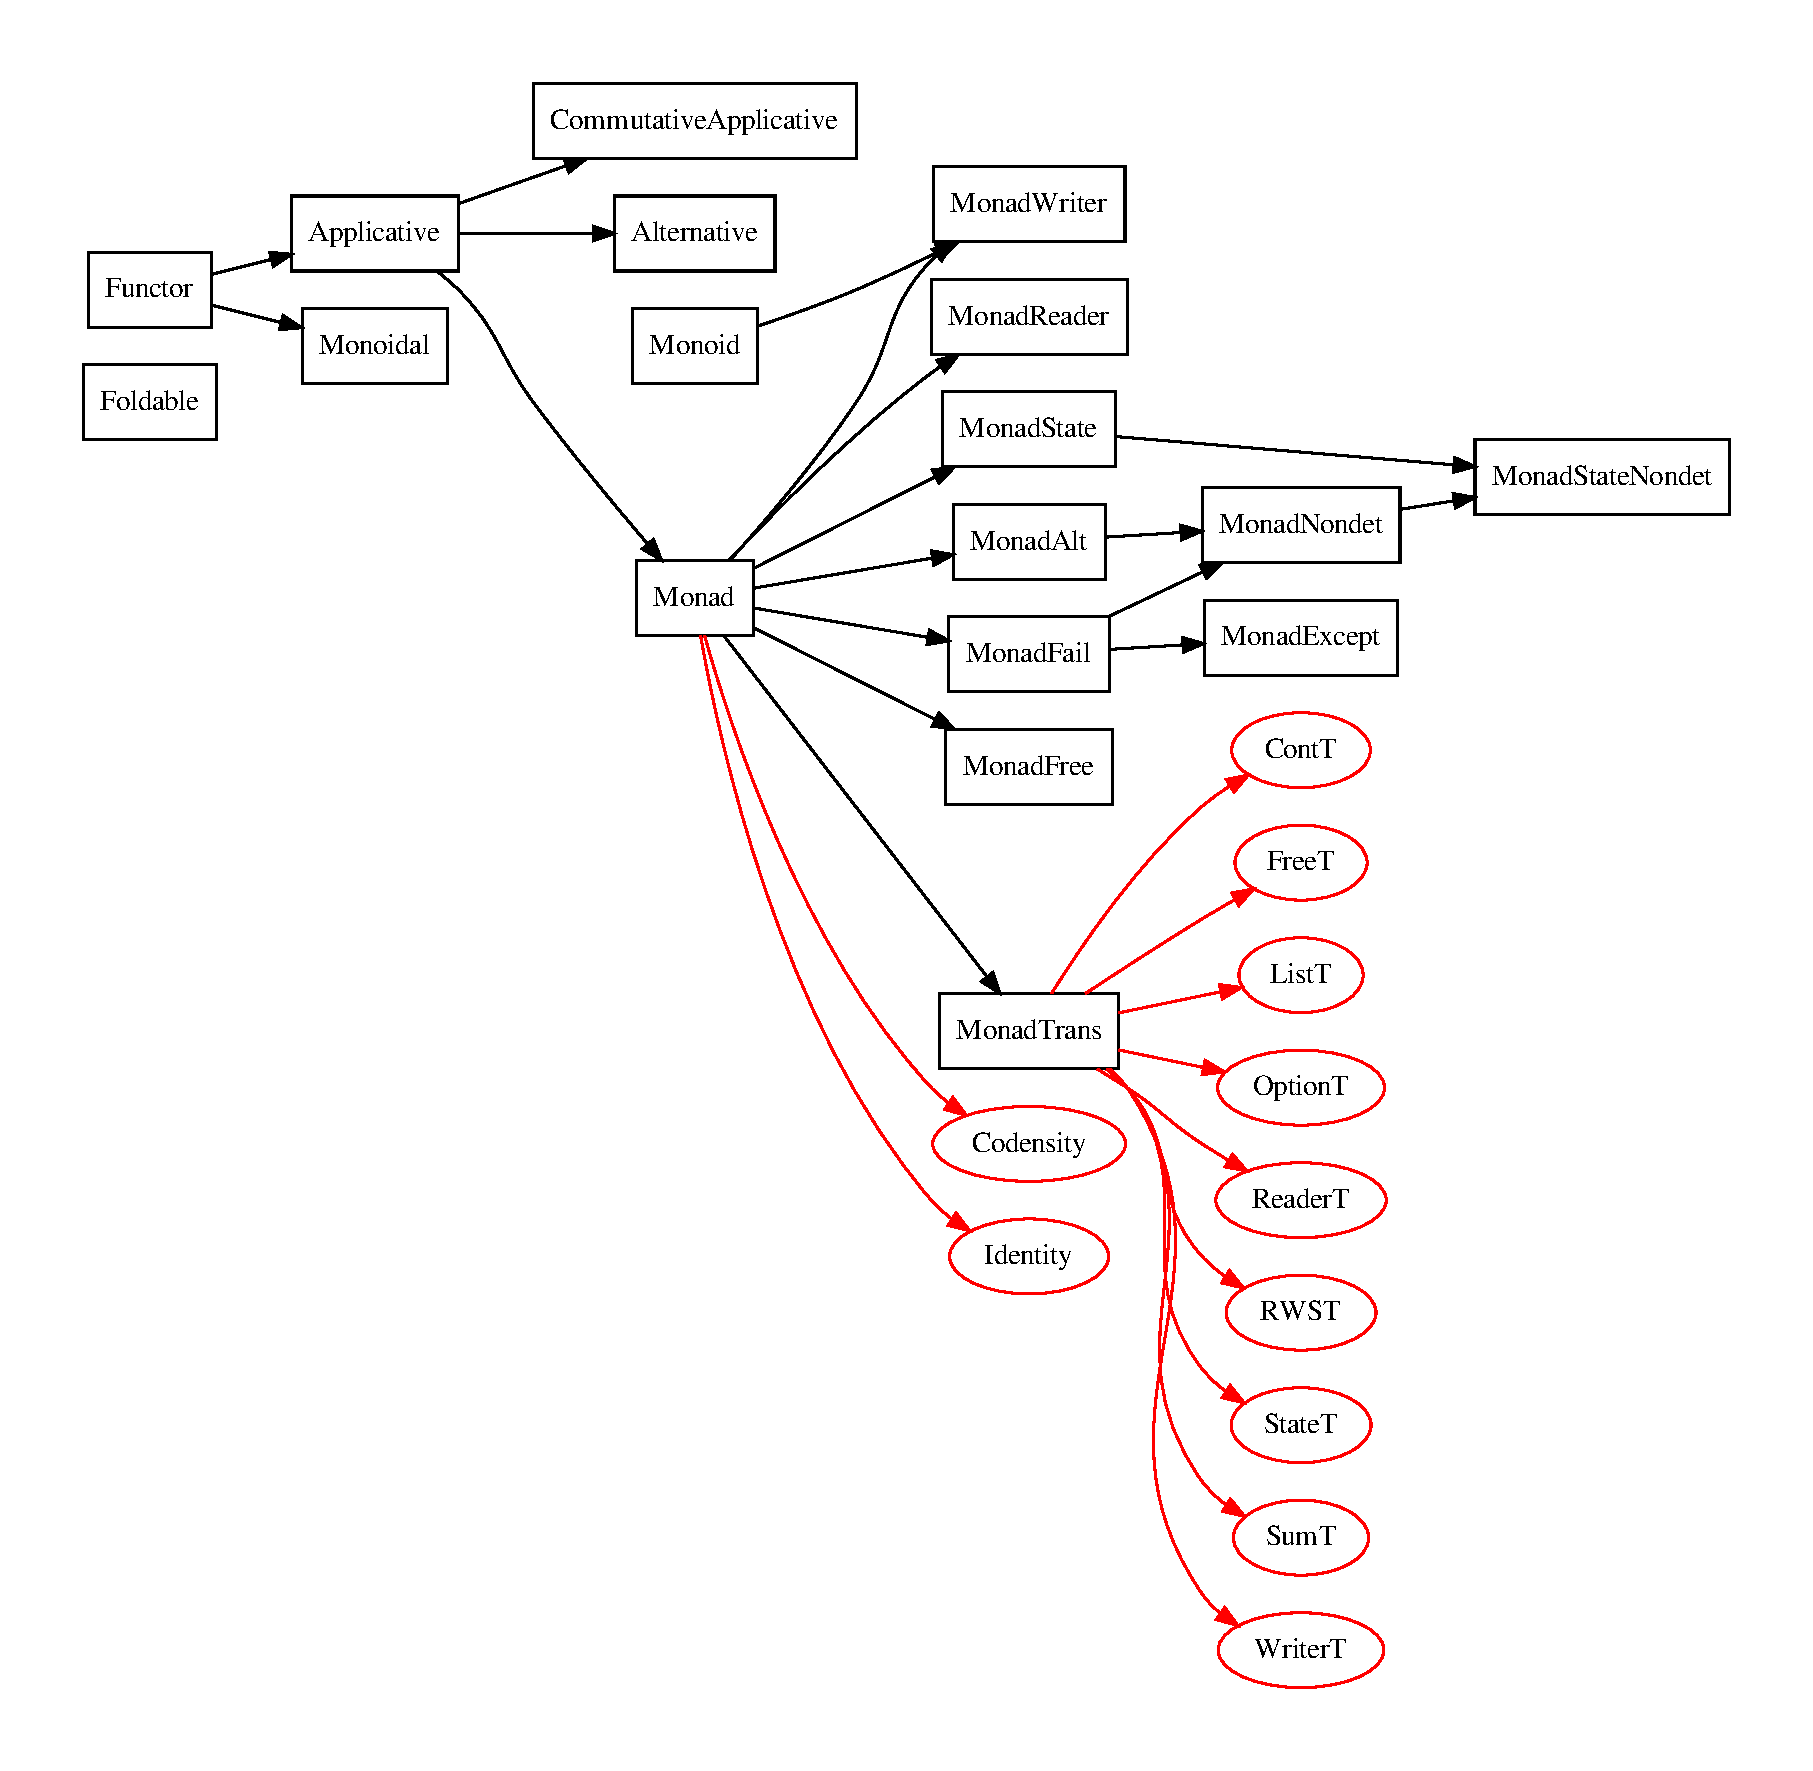
\includegraphics[width=20cm]{Hierarchy.pdf}}
    \caption{The library structure. Black boxes are classes, a black arrow from A to B means that class B depends on class A. Red ovals are class instances and a red arrow from A to B means that B is an instance of class A. A few classes were omitted (mainly variants of \m{MonadAlt}) and instances of the monadic effect classes (\m{MonadWriter} through \m{MonadFree}) were also omitted, as they would make the diagram unreadable.}
    \label{fig:hierarchy}
\end{figure}

\section{Axioms}

A very important property of every Coq development is being axiom free. The main reason is that the computational content of type theory is very axiom-sensitive. Because every axiom is just an element of some type, postulating it breaks the important property of canonicity. For example, if we postulate an axiom \m{nimber} of type \m{nat}, how does the term \m{nimber + 42} evaluate? The answer is that we don't know (or rather, it doesn't), because the definition of addition only handles the cases of zero and successor. This term is therefore stuck, i.e. it ``doesn't compute''.

\libname\ doesn't have the property of being axiom free. This is because a lot of monad laws (and other laws too), to be proved, require the Functional Extensionality Axiom, which states that two functions are equal as soon as they have equal results for all inputs. We therefore adopt this axiom from the very beginning and use it wherever we need it without explicit mention. The resulting loss of canonicity isn't that bad, however, because it only prevents us from performing some computations with equality proofs, which are not at all important. We therefore consider adopting this axiom to be justified.

\section{Proof engineering}

Now that we know our axioms, we can start proving, right? Well, not really. When programmers want to create something bigger than a toy program, they face the question of software engineering -- what architecture will be the best, what design will be the most robust, which tools to use etc. Writing assembly by hand or non-structured programming are not considered good software engineering practices anymore.

The same is true of mathematicians who go formal -- when they want to prove lots of theorems that form a coherent theory, they face the question of proof engineering -- what ``architecture'' will express best the structure of the theory, what style of proving will let them prove their theorems in the most painless way and so on. Writing proofterms by hand or simple proofscripts composed only of the most basic tactics are not good proof engineering practices. We should therefore stick with some good practices, but what are they?

Ltac, Coq's tactic language, is a very rich language and this has led to many proof styles being employed in various places. The most important distinction is between manual proofs (which consist of a series of tactics that prove the theorem step by step, like in the example in \hyperref[ch1]{Chapter 1}) and automated proofs (which usually take the form of a big tactic that proves a whole theorem all at once).

Another distinction is between reflective and non-reflective proofs. Reflective proofs are proofs written in Coq's term language that operate on syntactic representations of theorems. The sole role of Ltac in this approach is reification, i.e. transforming these theorems into their syntactic representations (this is something that Coq's term language cannot do, because it would result in inconsistency). Non-reflective proofs are the ordinary Ltac-based proofs that don't use the above machinery of reflection and reification. This gives rise to four proof styles:

\begin{itemize}
    \item Manual, non-reflective: often used by beginners and not considered a good practice, unless we're dealing with hard theorems that don't automate well.
    \item Manual, reflective: this is the style most associated with the SSReflect proof language \cite{SSReflect1} \cite{SSReflect2}, used in the formalization of the Four Colour Theorem \cite{FourColour1} \cite{FourColour2} and the Mathematical Components library \cite{MCB}.
    \item Automated, non-reflective: often used by experts for theorems with lots of repetitive cases or collections of similar theorems. An example is the field of programming language formalization, where proofs can have hundreds of cases, most of them utterly boring. A very known proponent of this style is Adam Chlipala, who advocates it in his book \cite{CPDT}.
    \item Automated, reflective: most often used for solving specific goals of a specific kind, like Presburger arithmetic (the arithmetic of natural numbers with addition and multiplication by a constant -- Coq's tactic \m{omega}) or simplifying expressions and proving equalities in rings (Coq's tactic \m{ring}).
\end{itemize}

In our case, there will be a massive amount of typeclass instances that have to be proven to satisfy the same laws over and over again. Almost all of these proofs are very repetitive and predictable. They amount mostly to unfolding definitions, rewriting equational laws, decomposing hypotheses and implicational reasoning. This means we want our proofs to be automated and not manual.

It may also seem that we want the tactics to be reflective, because the typeclasses we are dealing with are very well structured mathematically. This is however not the case, because we want our tactics to also be of use to users of our library, but we cannot predict what kinds of monads and effect they will want to create. This makes makes the world of \m{Functor}s, \m{Applicative}s, \m{Monad}s and effects not a closed world, like that of Presburger arithmetic or ring expressions, but an open one. We therefore choose to follow the automated non-reflective approach.

\chapter{Implementation, theorems and examples} \label{ch4}

In this chapter we describe the implementation of our library, including some subtleties that we didn't foresee coming during design, explain our approach to proof automation (how to prove all these laws without too much labor), give some example use cases of our library and prove a few theorems which may seem unnecessary at first, but turn out to have some practical use.

\section{The core library}

\begin{listing}[H]
    \inputminted
    [
        frame=lines,
        bgcolor=CoqIDE,
        linenos,
        firstline=8,
        lastline=16
    ]
    {Coq}{../Control/Functor.v}

    \caption{The \m{Functor} typeclass}
    \label{Functor}
\end{listing}

At the root of the library are, of course, functors, shown in listing \ref{Functor}. There should be nothing surprising to people who know them from Haskell, maybe except that the laws are now part of the definition. Note that we use \m{.>} to denote forward function composition, so that \m{f .> g} means \m{fun x => g (f x)}

A few category-theoretical remarks: unlike Haskell types and functions, which do \textit{not} form a category (see \cite{Hask} for details), Coq types and functions do form a category (or to be more precise, we can form a category whose objects are types from a given universe and morphisms are functions between them). The \m{Functor} typeclass represents endofunctors in this category. Note that all such functors \m{F} are strong in the sense that there is a morphism \m{strength : A -> F B -> F (A * B)}.

\begin{listing}[H]
    \inputminted
    [
        frame=lines,
        bgcolor=CoqIDE,
        linenos,
        firstline=11,
        lastline=34
    ]
    {Coq}{../Control/Applicative.v}

    \caption{The \m{Applicative} typeclass}
    \label{Applicative}
\end{listing}

The next step in the typeclass hierarchy are \m{Applicative} functors, shown in listing \ref{Applicative}. From the definition we see that an \m{Applicative} functor is a \m{Functor} into which we can inject a value (the function \m{pure}) and which allows to apply a function wrapped in the functor to an argument wrapped in the functor (the function \m{ap}, which is short for ``apply'').

These two operations, \m{pure} and \m{ap}, have to satisfy some laws and this is the first time that some subtle complications arise. The four laws that are usually presented (such as in \cite{LYAH}) are \m{identity}, \m{composition}, \m{homomorphism} and \m{interchange}. Other sources (like \cite{HackageApplicative} and \cite{WikibooksApplicative}) also mention a fifth law, \m{fmap\_pure\_ap}, but they often either state that this law follows from the other laws using naturality or they keep quiet about it.

In Coq naturality is not internalized (and in fact it can be broken by assuming classical axioms like the Law of Excluded Middle), so this law does not follow from the others. A more intuitive reason is that the other four laws don't mention any \m{Functor} concept at all, so there's no way to link \m{fmap} with \m{pure} and \m{ap} in any way. This is why we include this law in our definition.

This, however, leads to some further troubles, because it turns out that this set of five laws is not minimal. For example, \m{identity} follows from \m{fmap\_pure\_ap} and \m{fmap\_id} (for details, see the file \m{Theory/Laws/ApplicativeLaws.v}). It could lead us to drop \m{identity} from the definition of \m{Applicative}, but we decided not to.

\begin{listing}[H]
    \inputminted
    [
        frame=lines,
        bgcolor=CoqIDE,
        linenos,
        firstline=10,
        lastline=40
    ]
    {Coq}{../Control/Monoidal.v}

    \caption{The \m{Monoidal} typeclass}
    \label{Monoidal}
\end{listing}

Another question we could ask is: what are \m{Applicative} functors categorically? It is a sad question, because it gets answered rarely, but the answer is actually very simple -- \m{Applicative} functors are just \m{Monoidal} functors in disguise! The definition of a \m{Monoidal} functor is shown in listing \ref{Monoidal}. 

The category of Coq types and functions has a terminal object (the \m{unit} type) and binary products, which together (with some coherence conditions too) form its monoidal structure. A \m{Monoidal} functor (and thus, an \m{Applicative} functor) is a \m{Functor} which preserves this monoidal structure in the sense that \m{default}, \m{pairF}, \m{fmap fst}, \m{fmap snd} and \m{fmap reassoc} behave just like \m{tt} (the only value of the \m{unit} type), \m{pair}, \m{fst}, \m{snd} and \m{reassoc} and they do this in a natural way.

We have formally proved that \m{Applicative} and \m{Monoidal} are equivalent (see the file \m{Theory/Applicative\_is\_Monoidal.v}), which justifies the above explanation of the categorical semantics of \m{Applicative}. It also assures us that our set of \m{Applicative} laws is correct and that putting \m{fmap\_pure\_ap} in the definition was necessary.

But there is yet another perk of this proof, which shows that proving is not only of theoretical interest, but also has practical aspects -- thanks to this proof users of our library can now define an instance of either \m{Applicative} or \m{Monoidal} and get an instance of the other typeclass for free, something which is not possible in a language like Haskell.

\begin{listing}[H]
    \inputminted
    [
        frame=lines,
        bgcolor=CoqIDE,
        linenos,
        firstline=21,
        lastline=39
    ]
    {Coq}{../Control/Monad.v}

    \caption{The \m{Monad} typeclass}
    \label{Monad}
\end{listing}

Next come monads, shown in listing \ref{Monad}. The definition is very similar to modern Haskell, where \m{Applicative} is a superclass of \m{Monad} since GHC 7.10.1. The three usual laws are there, but there's also a fourth one, namely \m{bind\_ap} (this law is also mentioned in \cite{HackageMonad}).

The reason is that in the category of Coq types and functions each \m{Monad} is monoidal (in fact, the \m{Monad} typeclass represents a strong monoidal monad on the category of Coq types and functions), which means that it induces an instance of \m{Applicative}. However, it does so in two nonequivalent ways, which correspond to the two ways of defining \m{ap} using \m{bind} (which is sequential). To avoid potential doubling of \m{Monad} instances, we put the law \m{bind\_ap} in the definition, which forces \m{ap} to evaluate its arguments from left to right.

Just as in the \m{Applicative} case, an additional trouble is that this set of four laws is not minimal. For example, \m{bind\_pure\_l} follows from \m{fmap\_id}, \m{fmap\_pure\_ap}, \m{bind\_ap} and \m{bind\_pure\_l} -- see the file \m{Theory/Laws/MonadLaws.v} for details. We could have therefore dropped \m{bind\_pure\_l} from the definition, but we didn't decide to do so.

To make sure that this definition of monads makes sense, we proved that it is equivalent to a simpler one, which uses just \m{pure}, \m{bind} and the appropriate laws. We also prove it equivalent to a definition based on \m{Applicative}, but with \m{join} instead of \m{bind}. Of course these two equivalences can be used by the user to define an instance of whichever kind of \m{Monad} is the easiest for him and get the other ones for free.

Another interesting fact is that we also tried to prove this definition equivalent to one based on \m{pure} and \m{compM} (forward composition of monadic functions), which is closely related to the definition of a monad's Kleisli category, but we failed. See the directory \m{Theory/Equivs} for more details.

\begin{listing}[H]
    \inputminted
    [
        frame=lines,
        bgcolor=CoqIDE,
        linenos,
        firstline=60,
        lastline=73
    ]
    {Coq}{../Control/Monad.v}

    \caption{Monad notations}
    \label{MonadNotations}
\end{listing}

But what would monads be without their do-notation? As it turns out, we can define it using Coq's powerful notation mechanism, as shown in listing \ref{MonadNotations}. This do-notation is not perfect, because we need to follow each single \m{bind} with a semicolon and each use of \m{>>} (the operation that runs two computations in sequence, throwing away the result of the first) with a double semicolon. Also, the ``do'' part can be skipped without consequence, because it doesn't do anything. Despite these little annoyances, this do-notation works very well in practice.

It is also worth mentioning that our library contains all the usual utility functions associated with \m{Applicative} and \m{Monad}. In Haskell, these functions are often duplicated, with the \m{Applicative} version having the suffix \m{A} and the \m{Monad} version having the suffix \m{M}. In \libname\ these functions are deduplicated, i.e. there is always only one version of each, implemented using the weakest typeclass that suffices for the definition. See the files \m{Control/Applicative.v} and \m{Control/Monad.v} for their definitions.

\begin{listing}[H]
    \inputminted
    [
        frame=lines,
        bgcolor=CoqIDE,
        linenos,
        firstline=13,
        lastline=28
    ]
    {Coq}{../Control/Monad/Free.v}

    \caption{The \m{Free} monad}
    \label{Free}
\end{listing}

We have encountered problems that are not present in Haskell not only with the definitions of \m{Applicative}s and \m{Monad}s, but also when defining their instances. Coq, being a theorem prover, requires all inductive definitions to be strictly positive (i.e. the type being defined cannot stand to the left of an arrow or be applied to an opaque type-level function). This prevents us from defining the \m{Free} monad in the standard way, the problem being that the occurrence of \m{Free F A} is not strictly positive in \m{F (Free F A)}.

\begin{minted}
[
    frame=lines,
    bgcolor=CoqIDE,
    linenos
]{Coq}

Inductive Free (F : Type -> Type) (A : Type) : Type :=
| Pure : A -> Free F A
| Wrap : F (Free F A) -> Free F A.

\end{minted}

Our solution to this problem was to use Church encoding instead of inductive types. The resulting definition is shown in listing \ref{Free}. In this definition, we quantify over a type \m{X}, which represents the type we're defining, and then we put all the constructors into one big dependent function whose result is \m{X}.

This definition is fine in the sense that it allows us to define all necessary functions are prove all the laws. This may seem surprising, because it is well known that Church-encoded types don't support induction (i.e. their induction principles are not definable in Coq) \cite{InductionNotDerivable}. What's even more surprising is that they satisfy all these laws definitionally, i.e. we can prove all of them using just the tactic \m{reflexivity} -- see the proof of \m{Functor} laws in listing \ref{Free}.

Of course \m{Free} is not the only \m{Monad} instance. We provide all the standard ones: \m{Cont}, \m{Free}, \m{Identity}, \m{list}, \m{option}, \m{Reader}, \m{RWS}, \m{State}, \m{Sum}, \m{Writer} and there are also some less standard ones: \m{Codensity} (see \cite{ReflectionWithoutRemorse}), \m{Lazy} (which attempts to capture lazy evaluation in a monad) and \m{RoseTree} (a tree which keeps values only in its leaves).

\begin{listing}[H]
    \inputminted
    [
        frame=lines,
        bgcolor=CoqIDE,
        linenos,
        firstline=8,
        lastline=22
    ]
    {Coq}{../Control/Monad/Trans.v}

    \caption{The \m{MonadTrans} typeclass}
    \label{MonadTrans}
\end{listing}

The pinnacle of the core library are monad transformers, represented by the class \m{MonadTrans}, as shown in listing \ref{MonadTrans}. As we can see from the definition, a monad transformer is something which takes a monad and returns a monad, together with an operation \m{lift} that turns a base monad computation into a transformed monad computation, together with some obvious laws: \m{lift}ing a pure value has to result in a pure value, and \m{lift} has to commute with \m{bind}.

Luckily, monad transformers are just as unproblematic as \m{Functor}s were. The library implements all the standard instances, including \m{ContT}, \m{FreeT}, \m{ListT}, \m{OptionT}, \m{ReaderT}, \m{RWST}, \m{StateT}, \m{SumT} and \m{WriterT}.

\begin{listing}[H]
    \inputminted
    [
        frame=lines,
        bgcolor=CoqIDE,
        linenos,
        firstline=12,
        lastline=25
    ]
    {Coq}{../Control/Monad/Trans/ListT.v}

    \caption{ListT monad transformer}
    \label{ListT}
\end{listing}

The most noteworthy of these instances is \m{ListT}. Haskell's version of this monad transformer is broken (it doesn't respect the laws) and numerous solutions were proposed \cite{ListT1} \cite{ListT2} \cite{ListT3}. Our definition, shown in listing \ref{ListT}, follows \cite{ListT1} most closely, but once again we had to use Church encoding because the inductive version would fail the strict positivity criterion.

Thanks to Church encoding, all proofs (besides those that refer to the underlying monad) go through by \m{reflexivity} and this is a very strong sign that our \m{ListT} is really done right. Also thanks to Coq's notation mechanism, we can write \m{ListT} computations (\m{[[x; y; z]]}) nearly the same as we do ordinary lists (\m{[x; y; z]}).

\section{Proof engineering}

Are we so lucky that all proofs whatsoever go through just by \m{reflexivity}, like for the Church-encoded monads and monad transformers? Of course not -- most proofs require a bit more than just \m{reflexivity}.

This bit is surprisingly small -- the core of our automation is shown in listing \ref{Tactics}. The first ten lines are tactics for conveniently reasoning by functional extensionality (so that we can write \m{exts} instead of \m{extensionality a; extensionality b; ...}). Then comes the tactic \m{unmatch}, which destructs the innermost subject of a pattern match, and the tactic \m{destr}, which deconstructs products and units, and case splits on suns and subjects of pattern matching. \m{simplify} is a tactic that introduces variables to context, reasons by functional extensionality when it's possible and then calls \m{destr} to further simplify the goal.

\m{hs} is the main workhorse tactic of the library -- after introducing variables to the context, it proceeds by repeatedly unfolding definitions and rewriting equations and then tries to finish the goal off by unfolding a few more definitions and reasoning by \m{reflexivity} and \m{congruence} (which is an implementation of the congruence closure algorithm). At last, the \m{monad} tactic tries to simplify the goal, solve it using \m{hs} and if that isn't enough, then it tries some tricks for proving equations between monadic computations.

How does the rewriting and unfolding exactly work? It is quite simple: the tactics \m{autorewrite} and \m{autounfold} are called with some \textbf{hint databases} as arguments. For \m{autorewrite}, the hint database contains names of equations and for \m{autounfold} it contains names of defined objects. These tactics work by repeatedly rewriting/unfolding these equations/definitions in some order (determined by their implementations) until no more rewrites/unfoldings are possible.

Where do the hint databases come from? We have to create them and this is what line 29 in listing \ref{Tactics} does: it declares that the theorems named \m{id\_eq}, \m{id\_left}, \m{id\_right} belong to the hint database named \hintdb. Each time we encounter some useful equations (either in a typeclass definition or after proving them by hand), we add them to this hint database and from that point on \m{autorewrite} will be able to use them. We have to do the same for \m{autounfold}: each time we define something we will want to get unfolded, we add it to a hint database named \hintdb\ and from that point on \m{autounfold} will be able to unfold it for us.

Of course, these automation tactics are not enough to deal with all instances of all typeclasses. In a few cases we have to finish the proofs by hand. In a few other cases these tactics don't help us at all -- the most obvious example are lists, which require inductive proofs, but our tactics don't do any induction. The \m{Applicative} instance for lists is probably the most automation-resilient proof of the whole library. There are also a few proofs to which these tactics weren't even meant to apply, like the proof of equivalence of \m{Applicative} and \m{Monoidal} functors, which requires custom ad-hoc automation. Nonetheless, it's still surprising that some fifty lines of Ltac code can prove so many useful theorems.

\begin{listing}[H]
    \inputminted
    [
        frame=lines,
        bgcolor=CoqIDE,
        linenos,
        firstline=3,
        lastline=49
    ]
    {Coq}{../Thesis/snippets/Tactics.v}

    \caption{The automation tactics}
    \label{Tactics}
\end{listing}

\section{Typeclass-based effects}

We now describe ``typeclass-based effects'' (note that this is not a widely used term and, to be honest, we don't know if there is any widely used name for this approach to effects). Their popularity in Haskell is due to the \m{mtl} library (after which we also called this approach ``the \m{mtl} approach''), which was originally inspired by \cite{mtl}. Equational reasoning with such typeclass-based effects was first studied in \cite{JustDoIt}. This thesis is, to our knowledge, one of the earliest attempts to formalize this approach in Coq (with only \cite{MERC} being published earlier).

\begin{listing}[H]
    \inputminted
    [
        frame=lines,
        bgcolor=CoqIDE,
        linenos,
        firstline=6,
        lastline=12
    ]
    {Coq}{../Control/Monad/Class/MonadFail.v}

    \caption{The \m{MonadFail} typeclass}
    \label{MonadFail}
\end{listing}

In practice the whole thing works like this: each effect gets its own typeclass that lists all operations related to that effect and also equational laws that relate these operations to each other and to \m{pure} and \m{bind}. If a monad implements such a typeclass, it means that this monad supports that effect, i.e. it can be used to run programs that use that effect.

An example is shown in listing \ref{MonadFail}. This is one of the simplest possible effects -- failure. A monad that supports failure should provide an operation \m{fail} that is related to \m{bind} by the law \m{bind\_fail\_l}, which intuitively says that all computations following a failure also fail.

\begin{listing}[H]
    \inputminted
    [
        frame=lines,
        bgcolor=CoqIDE,
        linenos,
        firstline=6,
        lastline=15
    ]
    {Coq}{../Control/Monad/Class/MonadAlt.v}

    \caption{The \m{MonadAlt} typeclass}
    \label{MonadAlt}
\end{listing}

Another example, shown in listing \ref{MonadAlt}, is the \m{MonadAlt} typeclass, which represents the nondeterministic choice effect. A monad that supports this effect should provide an operation \m{choose} that is associative (the law \m{choose\_assoc}, which intuitively means that the various ways of associating a multiple choice don't make the choice biased) and left-distributes over \m{bind} (the law \m{bind\_choose\_l}, which intuitively means that a computation that depends on a choice is the same as a choice between computations).

\begin{listing}[H]
    \inputminted
    [
        frame=lines,
        bgcolor=CoqIDE,
        linenos,
        firstline=7,
        lastline=20
    ]
    {Coq}{../Control/Monad/Class/MonadNondet.v}

    \caption{The \m{MonadNondet} typeclass}
    \label{MonadNondet}
\end{listing}

A great strength of typeclass-based effects is that we can easily create new effects by composing previously defined effects and linking their operations with additional laws. An example is shown in listing \ref{MonadNondet}. The typeclass \m{MonadNondet} represents nondeterminism, understood as the ability to fail or make a binary choice (note that this is equivalent to being able to choose from a finite number of alternatives). The ``failure'' part comes from the \m{MonadFail} typeclass and the ``choice'' part comes from the \m{MonadAlt} typeclass. Moreover, there are two additional laws (\m{choose\_fail\_l} and \m{choose\_fail\_r}) which intuitively mean that we don't choose failure if we are not forced to.

\begin{listing}[H]
    \inputminted
    [
        frame=lines,
        bgcolor=CoqIDE,
        linenos,
        firstline=7,
        lastline=12
    ]
    {Coq}{../Control/Monad/Class/MonadReader.v}

    \caption{The \m{MonadReader} typeclass}
    \label{MonadReader}
\end{listing}

\begin{listing}[H]
    \inputminted
    [
        frame=lines,
        bgcolor=CoqIDE,
        linenos,
        firstline=35,
        lastline=45
    ]
    {Coq}{../Control/Monad/Class/MonadReader.v}

    \caption{The \m{MonadReader} instance for all monad transformers can be defined at once}
    \label{MonadReaderMonadTrans}
\end{listing}

But typeclass-based effects also have a great weakness which was already mentioned -- they require a quadratic amount of instances to be defined (in \m{mtl} the formula is the number of typeclasses times the number of monad transformers). In \libname\ the situation is very similar, but surprisingly, there is a single exception -- the \m{MonadReader} typeclass, shown in listing \ref{MonadReader}.

It represents a very simple effect that lets us \m{ask} the environment for a value of type \m{R}. The law \m{ask\_ask} states that asking twice is the same as asking just once. Because this typeclass is so simple, it turns out we can define a \m{MonadReader} instance for all monad transformers in one fell swoop, something that is not possible in Haskell. This reduces the amount of boilerplate we have to write, even though the amount of instances is still quadratic, and gives some hope that maybe this will be possible for other kinds of effect typeclasses. This hope is in vain however, as we empirically checked that this trick doesn't work even for other very simple effects, like \m{MonadFail}.

We have implemented most typeclasses that appear in \cite{JustDoIt}, including \m{MonadExcept}, \m{MonadFail}, \m{MonadAlt} (and its variants \m{MonadAltBag}, \m{MonadAltSet} and \m{MonadAlt2}), \m{MonadNondet}, \m{MonadState}, \m{MonadStateNondet}, but we omitted the probability monad. We have also formalized most of \cite{JustDoIt} -- see the file \m{Theory/JustDoIt.v} for details.

We have also implemented a few effect typeclasses that should be familiar from \m{mtl}, like \m{MonadReader}, \m{MonadWriter} and \m{MonadFree}, but there are some differences: as we have seen, \m{MonadReader} lacks the \m{local} operation that is present in \m{mtl} and it was quite hard to figure out the ``correct'' laws that \m{MonadWriter} instances should obey (what we did was empirically test which laws were satisfied by most instances and adopted these).

\begin{listing}[H]
    \inputminted
    [
        frame=lines,
        bgcolor=CoqIDE,
        linenos,
        firstline=14,
        lastline=29
    ]
    {Coq}{../Control/Monad/Class/MonadState.v}

    \caption{The \m{MonadState} typeclass}
    \label{MonadState}
\end{listing}

\section{Examples}

We finish this chapter with two examples of reasoning with our monads and effects. First we revisit the example from \hyperref[ch1]{Chapter 1} and see how it can be improved with do-notation and automation tactics. We finish with a formalization of the fast product example from \cite{JustDoIt}.

\subsection{Tree labeling, again}

The tree labeling example is shown in listing \ref{Example1}. The definitions of \m{Tree} and \m{size} are as before, so they are omitted. We want to implement the \m{label} function using the state effect, so we start by importing the \m{MonadState} typeclass, shown in listing \ref{MonadState}. The state effect supports two operations, \m{get} and \m{put}, which are related by four very intuitive laws -- we encourage the reader to figure out that they mean.

The \m{label} function looks very different than before. Its type is more complicated now, because we have generalized it to work for any monad supporting the \m{MonadState} effect. However, the body of the definition is much easier to read because of do-notation. 

The function works just like before. If we hit a \m{Leaf}, we retrieve the state of the counter and use it to label the \m{Leaf}. If we hit a \m{Node}, we label the left subtree, increase the counter by one (\m{modify S} means ``modify the state by applying the function \m{S}'', which is the successor function), label the right subtree and then we join these two labeled subtrees with \m{Node}.

To get the function we really want (\m{lbl}, which starts labeling from zero) we have to instantiate the definition of \m{label} with some monad supporting the state effect and we of course choose the \m{State} monad. We see that we can compute with this definition just like we could with the old one and the result is, of course, the same.

The correctness theorem (which states that after running \m{label} on a tree \m{t}, the counter increases by the size of \m{t}) looks quite similar the old one, just as does the proof. There are two important things to notice. First, we prove this theorem only for the concrete \m{State} monad and not for any monad supporting the \m{MonadState} effect. This is because the state effect doesn't give us any way of pulling the state outside the monad and we need this ability to even state the theorem. Second, we crucially use our automation tactic \m{hs}, which changes the proof state from barely readable (it mentions the particular definitions of \m{pure}, \m{bind} and so on for the \m{State} monad) to one that strongly resembles the earlier, non-monadic version from \hyperref[ch1]{Chapter 1}.

The overall result is that the \m{label} function is more general, its definition is easier to read and the proof didn't get any harder. Not bad.

\begin{listing}[H]
    \inputminted
    [
        frame=lines,
        bgcolor=CoqIDE,
        linenos,
        firstline=16,
        lastline=53
    ]
    {Coq}{../Thesis/snippets/Example1.v}

    \caption{The tree labeling example from \hyperref[ch1]{Chapter 1}, generalized with the \m{MonadState} typeclass and improved with do-notation}
    \label{Example1}
\end{listing}

\subsection{Fast product}

A fast product is a procedure for calculating the product of a list that returns zero as soon as it encounters a zero on this list, without having to consider the rest of the list. We will implement it using exceptions, so first we have to introduce the \m{MonadExcept} effect, shown in listing \ref{MonadExcept}.

\begin{listing}[H]
    \inputminted
    [
        frame=lines,
        bgcolor=CoqIDE,
        linenos,
        firstline=14,
        lastline=31
    ]
    {Coq}{../Control/Monad/Class/MonadExcept.v}

    \caption{The \m{MonadExcept} typeclass}
    \label{MonadExcept}
\end{listing}

The only exception that monads supporting the \m{MonadExcept} effect can throw is \m{fail}, inherited from the \m{MonadFail} effect. \m{MonadExcept} additionally provides an operation \m{catch} for catching these exceptions. \m{fail} and \m{catch} are related by four laws: they form a monoid (\m{catch\_fail\_l}, \m{catch\_fail\_r} and \m{catch\_assoc}, which intuitively mean that, respectively, failing computations are caught, failing handlers are not used and that the nesting of exception handlers doesn't matter), and they also obey the law \m{catch\_pure} which says that handlers are not used for computations that don't fail. The laws of \m{MonadFail} are of course inherited too.

Note that the operations supported by \m{MonadExcept} (\m{fail} and \m{catch}) have the same types as those supported by \m{MonadNondet} (\m{fail} and \m{choose}), but their intended meaning is very different, as captured by the laws. It is therefore the operations together with the laws that determine the meaning of an effect, not just the operations alone.

\begin{listing}[H]
    \inputminted
    [
        frame=lines,
        bgcolor=CoqIDE,
        linenos,
        firstline=269,
        lastline=307
    ]
    {Coq}{../Theory/JustDoIt.v}

    \caption{The fast product example}
    \label{Example2}
\end{listing}

We now proceed to the example, shown in listing \ref{Example2}. Not shown are the functions \m{product}, which computes the product of a list of natural numbers, \m{has}, which checks if a natural number is present in a list and the proof of the lemma \m{product\_has\_0}, which says that if a zero appears in a list, then the product of that list is equal to zero.

We now define a function \m{work}, which works for any monad which supports the failure effect. It checks if a list contains a zero and fails if it does and calls \m{product} otherwise. Using this auxiliary function we define \m{fastprod}, which wraps \m{work} in a handler that just returns zero in case of failure.

The correctness of \m{fastprod} is stated as theorem \m{fastprod\_spec}, which says that \m{fastprod} is equal to a pure computation that just calls \m{product}. The proof is very simple. We unfold the definitions of \m{fastprod} and \m{work}, introduce variables to context and perform a case split on whether the list contains a zero. In both subcases we use the laws of \m{MonadExcept} (together with the lemma \m{product\_has\_0} in the first case) to conclude that the result is the same as a pure computation using \m{product}.

This may look unimpressive, because \m{work} is implemented using a simple case split, without recursion. We could also implement \m{work} recursively, by checking if the head of the list is zero and failing in this case, otherwise multiplying the product of the tail by the head.

The theorem \m{work\_foldr} states that \m{work} is equal to a function implemented precisely this way (but using \m{fold\_right} instead of pattern matching). The proof is also very simple: we reason by functional extensionality and then by induction. The empty list case is simple. In the \m{cons} case we reason by cases on whether the head of the list is zero. In both cases we finish by using some \m{Monad} and \m{MonadFail} laws together with the induction hypothesis.

The above proof is as simple as the pen-and-paper one that can be found in \cite{JustDoIt} in section 5.1 (even though the line of reasoning is a bit different). This shows that at least for simple theorems our library doesn't induce a ``formalization overhead''.

\chapter{Conclusion} \label{ch5}

We have introduced \libname, a Coq library for formally verified programming with Haskell-style abstractions. We have centered our presentation on the matter effects, with which we dealt by implementing a collection of \m{mtl}-like abstractions whose main inspiration was \cite{JustDoIt}.

In \hyperref[ch1]{Chapter 1} we gave some arguments for why formal verification is worth pursuing and introduced the Coq proof assistant. In \hyperref[ch2]{Chapter 2} we explained the basics of computational effects and outlined the main approaches. In \hyperref[ch3]{Chapter 3} we elucidated the design choices, which weren't really that many, described the implementation and explained the mechanism behind our proof automation. In \hyperref[ch4]{Chapter 4}, we have formalized some examples from \cite{JustDoIt} to show the viability of the library. We also saw some simple theorems which prove our implementation correct, but are also useful from a practical point of view.

\section{Technical details}

The source code and build instructions for \libname\ and the source code of this thesis can be found at \homepage. The code is extensively commented and this is the only available kind of documentation. Pull requests and suggestions are welcome.

\section{Related work}

There has been relatively little work on effects in Coq. \cite{MERC} is another attempt at an \m{mtl}-like library for Coq. It is similar to our work by also drawing inspiration from \cite{JustDoIt}, but differs in technical details (it uses canonical structures instead of classes) and focus (their motivation is formalization of programming languages).

There is an implementation of effects in Coq, available at \cite{CoqIO}, that allows one to define programs with IO and even concurrency and then extract the code to OCaml. This development is, however, rather obscure (there is not even a single paper about it). There also is an implementation of exceptions by means of a translation from the Calculus of Constructions to itself, realized in Coq as a plugin \cite{FailureIsNotAnOption}.

Besides, there has been some work on formally verifying programs with algebraic effects and handlers in Coq \cite{CoqEff1} \cite{CoqEff2} and more generally, on effectful programming in Coq \cite{CoqEff3}.

Among dependently typed languages most similar to Coq, there has been some work on an effect system for Idris \cite{IdrisEffects}. Another languages that mixes dependent types and effects (and also refinement types) is F* \cite{FStar}.

\section{Further work}

There's still some work to be done. The TODO list can be found by looking at the \m{TODO} section in \m{README.md} and by searching the source code for the keywords \m{Abort}, \m{Admitted} and for the marker TODO.

First off, some proofs and instances are missing. For example, I could neither define an instance of \m{MonadExcept} for \m{FreeT} nor prove that none exists. The same is true for a few more transformer/class pairs.

Notations could get some love too. The current do notation requires the ugly \m{;;} for computations that don't bind their result and I couldn't even define the idiom brackets of Idris using Coq's notation mechanism.

Some more theoretical work would be to formally characterize the minimal sets of laws for the various classes and some more practical work would be to implement other useful abstractions known from Haskell, like \m{Traversable}.

Another possibility is to rewrite the whole automation engine, so as to use proof by reflection \cite{CPDT}, which is more reliable than the more ad hoc tactics written in Ltac. The first step toward this goal has already been made with the tactic \m{reflect\_functor}, which implements basic principles of reasoning with functors.

Last but not least, as already mentioned, \libname\ is a basis on which a library similar to Haskell's \m{extensible-effects} may be implemented.

%%%%% BIBLIOGRAFIA

\begin{thebibliography}{1}

    \bibitem{JustDoIt}
        Jeremy Gibbons and Ralf Hinze, \\
        \textit{Just do It: Simple Monadic Equational Reasoning}, 2011 \\
        \url{http://www.cs.ox.ac.uk/jeremy.gibbons/publications/mr.pdf}

    \bibitem{Meltdown}
        Moritz Lipp, Michael Schwarz, Daniel Gruss, Thomas Prescher, Werner Haas, Anders Fogh, Jann Horn, Stefan Mangard, Paul Kocher, Daniel Genkin, Yuval Yarom and Mike Hamburg, \\
        \textit{Meltdown: Reading Kernel Memory from User Space}, 2018 \\
        \url{https://meltdownattack.com/meltdown.pdf}

    \bibitem{Spectre}
        Paul Kocher, Jann Horn, Anders Fogh, Daniel Genkin, Daniel Gruss, Werner Haas, Mike Hamburg, Moritz Lipp, Stefan Mangard, Thomas Prescher, Michael Schwarz and Yuval Yarom, \\
        \textit{Spectre Attacks: Exploiting Speculative Execution}, 2019 \\
        \url{https://spectreattack.com/spectre.pdf}
    
    \bibitem{Heartbleed}
        \url{https://heartbleed.com}

    \bibitem{DeepSpec}
        \url{https://deepspec.org}

    \bibitem{Boeing}
        Gregory Travis, \\
        \textit{How the Boeing 737 Max Disaster Looks to a Software Developer}, \\
        \url{https://spectrum.ieee.org/aerospace/aviation/how-the-boeing-737-max-disaster-looks-to-a-software-developer}
    
    \bibitem{AppelHaken1}
        Kenneth Appel, Wolfgang Haken,
        \textit{Every map is four colorable}, 1976, \\
        \url{https://pdfs.semanticscholar.org/3d50/72364f230e1ab5a0b3725d84d15689615077.pdf}
    
        \bibitem{AppelHaken2}
        Kenneth Appel, Wolfgang Haken, \\
        \textit{Every planar map is four colorable. Part I: Discharging}, 1977, \\
        \url{https://projecteuclid.org/euclid.ijm/1256049011}

    \bibitem{AppelHaken3}
        Kenneth Appel, Wolfgang Haken, \\
        \textit{Every  map  is  four  colorable,  Part  II:  Reducibility}, 1977, \\
        \url{https://projecteuclid.org/euclid.ijm/1256049012}

    \bibitem{AppelHaken4}
        Kenneth Appel, Wolfgang Haken,
        \textit{Every  map  is  four  colorable}, 1989, \\
        \url{https://bookstore.ams.org/conm-98}

    \bibitem{NonSurveyable}
        Thomas Tymoczko, \\
        \textit{The Four-Color Problem and Its Philosophical Significance}, 1979, \\
        \url{http://thatmarcusfamily.org/philosophy/Course_Websites/Math_S08/Readings/tymoczko.pdf}

    \bibitem{FourColour1}
        Georges Gonthier,
        \textit{A computer-checked proof of the Four Colour Theorem}, 2005 \\
        \url{https://www.cl.cam.ac.uk/~lp15/Pages/4colproof.pdf}
    
    \bibitem{FourColour2}
        Georges Gonthier,
        \textit{Formal Proof -- The Four-Color Theorem}, 2008, \\
        \url{http://www.ams.org/notices/200811/tx081101382p.pdf}

    \bibitem{UnivalentFoundations}
        Vladimir Voevodsky,
        \textit{UNIVALENT FOUNDATIONS}, \\
        slides for a talk given at IAS on 26 March 2014, \\
        \url{http://www.math.ias.edu/~vladimir/Site3/Univalent_Foundations_files/2014_IAS.pdf}

    \bibitem{Coq}
        \url{https://coq.inria.fr/}

    \bibitem{CurryHoward}
        Morten Heine Sørensen, Paweł Urzyczyn, \\
        \textit{Lectures on the Curry-Howard Isomorphism}, 2006, \\
        \url{http://disi.unitn.it/~bernardi/RSISE11/Papers/curry-howard.pdf}
    
    \bibitem{SoftwareFoundations}
        Benjamin C. Pierce, Andrew W. Appel et al, \\
        \textit{Software Foundations}, 2019, \\
        \url{https://softwarefoundations.cis.upenn.edu/}
    
    \bibitem{CoqArt}
        Yves Bertot and Pierre Castéran, \\
        \textit{Interactive Theorem Proving and Program Development \\ Coq'Art: The Calculus of Inductive Constructions}, 2004, \\
        \url{https://www.labri.fr/perso/casteran/CoqArt/}

    \bibitem{CPDT}
        Adam Chlipala,
        \textit{Certified Programming with Dependent Types}, \\
        \url{http://adam.chlipala.net/cpdt/}

    \bibitem{BillionDollarMistake}
        Tony Hoare,
        \textit{Null References: The Billion Dollar Mistake}, \\
        \url{https://www.infoq.com/presentations/Null-References-The-Billion-Dollar-Mistake-Tony-Hoare/}
    
    \bibitem{CWM}
        Saunders Mac Lane,
        \textit{Categories for the Working Mathematician}, 1971, \\
        \url{http://books.google.com/books?id=MXboNPdTv7QC&pg=PA138&lpg=PA138&dq=%22monoid+in+the+category+of+endofunctors%22+mac+lane&source=bl&ots=feQWTkH2Uw&sig=tv-1JwaMOygKGmFE2vM2FhJVS9o&hl=en&ei=5iWsTJCkBIPSsAPQwJ36Aw&sa=X&oi=book_result&ct=result&resnum=1&ved=0CBIQ6AEwAA#v=onepage&q&f=false}

    \bibitem{MonadTutorialFallacy}
        Brent Yorgey, \textit{Abstraction, intuition, and the ``monad tutorial fallacy''}, \\
        \url{https://byorgey.wordpress.com/2009/01/12/abstraction-intuition-and-the-monad-tutorial-fallacy/}

    \bibitem{Moggi}
        Eugenio Moggi,
        \textit{Notions of computation and monads}, 1991, \\
        \url{https://person.dibris.unige.it/moggi-eugenio/ftp/ic91.pdf}

    \bibitem{mtl}
        Mark P. Jones, \\
        \textit{Functional Programming with Overloading and Higher-Order Polymorphism}, 1995, \\
        \url{http://web.cecs.pdx.edu/~mpj/pubs/springschool95.pdf}

    \bibitem{ExtensibleEffects}
        Oleg Kiselyov, Amr Sabry, Cameron Swords, \\
        \textit{Extensible Effects. An Alternative to Monad Transformers}, 2013, \\
        \url{http://okmij.org/ftp/Haskell/extensible/exteff.pdf}

    \bibitem{Freer}
        Oleg Kiselyov, Hiromi Ishii, \\
        \textit{Freer Monads, More Extensible Effects}, \\
        \url{http://okmij.org/ftp/Haskell/extensible/more.pdf}

    \bibitem{Koka}
        Daan Leijen,
        \textit{Koka: Programming with Row Polymorphic Effect Types}, 2014, \\
        \url{https://www.microsoft.com/en-us/research/wp-content/uploads/2016/02/paper-20.pdf}

    \bibitem{Eff}
        \url{https://www.eff-lang.org/}

    \bibitem{Frank}
        Sam Lindley, Connor McBride, \textit{Do Be Do Be Do}, 2014, \\
        \url{http://homepages.inf.ed.ac.uk/slindley/papers/frankly-draft-march2014.pdf}

    \bibitem{MulticoreOCaml}
        \url{https://github.com/ocaml-multicore/ocaml-multicore}
        
    \bibitem{Helium}
        \url{https://bitbucket.org/pl-uwr/helium/src/master/}

    \bibitem{CoqIO}
        \url{https://coq.io}

    \bibitem{Agda}
        \url{https://github.com/agda/agda}

    \bibitem{Idris}
        \url{https://www.idris-lang.org/}

    \bibitem{MERC}
        Reynald Affeldt, David Nowak, \\
        \textit{Experimenting with Monadic Equational Reasoning in Coq}, 2018, \\
        \url{http://jssst.or.jp/files/user/taikai/2018/PPL/ppl2-2.pdf}

    \bibitem{FailureIsNotAnOption}
        Pierre-Marie Pédrot, Nicolas Tabareau \\
        \textit{Failure is Not an Option: An Exceptional Type Theory}, 2018, \\
        \url{https://link.springer.com/chapter/10.1007/978-3-319-89884-1_9}

    \bibitem{CoqEff1}
        Jean-Guillaume Dumas, Dominique Duval, Burak Ekici, Damien Pous \\
        \textit{Formal verification in Coq of program properties involving the global state effect}, 2014, \\
        \url{https://hal.archives-ouvertes.fr/file/index/docid/872324/filename/DDEP-coqstates.pdf}

    \bibitem{CoqEff2}
        Thomas Letan, Yann Régis-Gianas, Pierre Chifflier, Guillaume Hiet, \\
        \textit{Modular Verification of Programs with Effects and Effect Handlers in Coq}, 2018, \\
        \url{https://hal.inria.fr/hal-01799712/document}

    \bibitem{CoqEff3}
        Greg Morrisett,
        \textit{Programming with Effects in Coq}, 2008, \\
        \url{https://link.springer.com/chapter/10.1007%2F978-3-540-70594-9_3}

    \bibitem{IdrisEffects}
        Edwin C. Brady, \\
        \textit{Programming and Reasoning with Algebraic Effects and Dependent Types}, 2013, \\
        \url{https://eb.host.cs.st-andrews.ac.uk/drafts/effects.pdf}

    \bibitem{FStar}
        \url{https://www.fstar-lang.org/}
    
    \bibitem{Classes1}
        Matthieu Sozeau, Nicolas Oury,
        \textit{First-Class Type Classes}, \\
        \url{https://www.irif.fr/~sozeau/research/publications/First-Class_Type_Classes.pdf}

    \bibitem{Classes2}
        \url{https://coq.inria.fr/distrib/current/refman/addendum/type-classes.html}

    \bibitem{CanonicalStructures0}
        Amokrane Saïbi, \\
        \textit{Outils Génériques de Modélisation et de Démonstration pour la Formalisation des Mathématiques en Théorie des Types. Application à la Théorie des Catégories.}, 1998, \\
        \url{https://tel.archives-ouvertes.fr/tel-00523810/file/Saibi_-_1999_-_Outils_GA_nA_riques_de_modA_lisation_et_de_dA_monstration_pour_la_Formalisation_des_MathA_matiques_en_thA_orie_des_Types_Application_A_la_thA_orie_des_catA_gories.pdf}

    \bibitem{CanonicalStructures1}
        Georges Gonthier, Beta Ziliani, Aleksandar Nanevski, Derek Dreyer, \\
        \textit{How to make ad hoc proof automationless ad hoc}, 2013, \\
        \url{https://software.imdea.org/~aleks/papers/lessadhoc/journal.pdf}

    \bibitem{CanonicalStructures2}
        Assia Mahboubi, Enrico Tassi, \\
        \textit{Canonical Structures for the working Coq user}, 2013, \\
        \url{https://hal.inria.fr/hal-00816703v2/document}

    \bibitem{CanonicalStructures3}
        \url{https://coq.inria.fr/refman/addendum/canonical-structures.html}

    \bibitem{MCB}
        Assia Mahboubi and Enrico Tassi with contributions by Yves Bertot and Georges Gonthier, \\
        \textit{Mathematical Components}, 2018, \\
        \url{https://math-comp.github.io/mcb/}

    \bibitem{Modules1}
        Jacek Chrząszcz,
        \textit{Modules in Coq Are and Will Be Correct}, 2004, \\
        \url{https://link.springer.com/chapter/10.1007%2F978-3-540-24849-1_9}

    \bibitem{Modules2}
        \url{https://coq.inria.fr/distrib/current/refman/language/module-system.html}

    \bibitem{Hask}
        \url{https://wiki.haskell.org/Hask}

    \bibitem{LYAH}
        Miran Lipovača,
        \textit{Learn You a Haskell for Great Good}, 2011, \\
        \url{http://learnyouahaskell.com/functors-applicative-functors-and-monoids#applicative-functors}

    \bibitem{HackageApplicative}
        \url{https://hackage.haskell.org/package/base-4.12.0.0/docs/Control-Applicative.html}

    \bibitem{WikibooksApplicative}
        \url{https://en.wikibooks.org/wiki/Haskell/Applicative_functors}

    \bibitem{HackageMonad}
        \url{https://hackage.haskell.org/package/base-4.12.0.0/docs/Control-Monad.html}

    \bibitem{InductionNotDerivable}
        Herman Geuvers, \\
        \textit{Induction Is Not Derivable in Second Order Dependent Type Theory}, 2001, \\
        \url{https://link.springer.com/chapter/10.1007/3-540-45413-6_16}

    \bibitem{ReflectionWithoutRemorse}
        Atze van der Ploeg, Oleg Kiselyov, \\
        \textit{Reflection without Remorse}, 2014, \\
        \url{http://okmij.org/ftp/Haskell/zseq.pdf}

    \bibitem{ListT1}
        \url{https://wiki.haskell.org/ListT_done_right}

    \bibitem{ListT2}
        \url{https://wiki.haskell.org/ListT_done_right_alternative}

    \bibitem{ListT3}
        \url{https://hackage.haskell.org/package/list-t}

    \bibitem{SSReflect1}
        Georges Gonthier, Assia Mahboubi, Enrico Tassi \\
        \textit{A Small Scale Reflection Extension for the Coq system}, 2016, \\
        \url{https://hal.inria.fr/inria-00258384v17/document}

    \bibitem{SSReflect2}
        \url{https://coq.inria.fr/refman/proof-engine/ssreflect-proof-language.html}
\end{thebibliography}

%\begin{thebibliography}{1}
%\bibitem{example} \ldots
%\end{thebibliography}

\end{document}